% 项目用到的技术与工具简介

\documentclass[UTF8]{ctexbook}
%
  \ctexset{
      part/number = \chinese{part}% 用于解决 part 的标号不显示问题
  }
  \usepackage{hyperref}% 超链接
  \hypersetup{
      colorlinks=false,% 去掉超链接颜色
      pdfborder=0 0 0% 取消超链接的边框
  }
  \usepackage{graphicx}% 图片管理
  \graphicspath{{images/}}% 设置图片搜索路径
  \usepackage{float,varwidth}% 浮动体
  \usepackage{booktabs}% 三线表
  \usepackage{tabularx}% 让表格自适应宽度与自动换行
  \newcolumntype{Y}{>{\centering\arraybackslash}X}% 定义自适应列的居中格式 Y, 用 X 为左对齐(自适应列)
  \usepackage{fancyhdr}% 页眉设置
  \usepackage{xcolor}% 颜色宏包
  \usepackage{listings}% 代码高亮
  \definecolor{codegreen}{rgb}{0,0.6,0}
  \definecolor{codegray}{rgb}{0.5,0.5,0.5}
  \definecolor{codepurple}{rgb}{0.58,0,0.82}
  \definecolor{backcolour}{rgb}{0.95,0.95,0.92}
  \lstset{
      commentstyle=\color{codegreen},
      keywordstyle=\color{magenta},
      stringstyle=\color{codepurple},
      basicstyle=\footnotesize,% 代码字体大小
      breakatwhitespace=false,% 是否只在空白字符处断行
      breaklines=true,% 自动断行
      captionpos=b,% 标题位置为 bottom
      keepspaces=true,
      numbers=left,% 行号的位置
      numbersep=5pt,% 行号与代码的距离
      numberstyle=\tiny\color{codegray},% 行号样式
      stepnumber=2,% 隔行显示行号
      showspaces=false,
      showstringspaces=false,
      showtabs=false,
      tabsize=2
  }
\begin{document}
  \chapter{技术、框架与工具}
    \label{chap:技术与工具}
      本章主要介绍了项目所用到的技术和工具,技术包括:
      \begin{itemize}
        \item HTTP
        \item JSON 与 XML
        % \item Apache 服务器的配置
        % \item Nodejs 与 npm
        \item MongoDB
        \item H5
        \item CSS3
        \item Less
        \item ES5,ES6
        \item jquery
        \item MVC
        \item AngularJS
      \end{itemize}

      工具包括:

      \begin{itemize}
        \item Sublime Text3
        \item Chrome
        \item 微信 Web 开发者工具
        \item Git
      \end{itemize}

    \section{技术与框架}
      \label{sec:技术框架}

        \subsection{HTTP}
          \label{subsec:http}
            \subsection{原理}
              \label{subsec:原理}
              什么是 HTTP

        \subsection{AngularJS}
          \label{subsec:angularjs}

            AngularJS 开发的应用是单页面应用,即 SPA(Single Page Applicaiton),单页应用的特点可以简单的概括为:模板 + 路由。只需一个入口 html 文件引入页面的基本结构以及所有的资源,如图 \ref{fig:index},
            \begin{figure}[H]
              \centering
              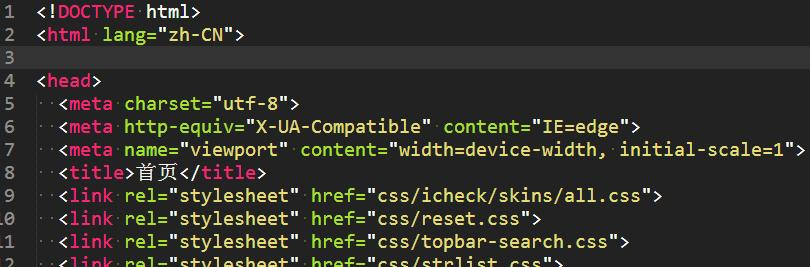
\includegraphics[width=10cm]{./img/index.jpg}
              \caption{入口页示例}
              \label{fig:index}
            \end{figure}

            其他的页面只需写入 html 片段即可, 如图 \ref{fig:tpl}

            \begin{figure}[H]
              \centering
              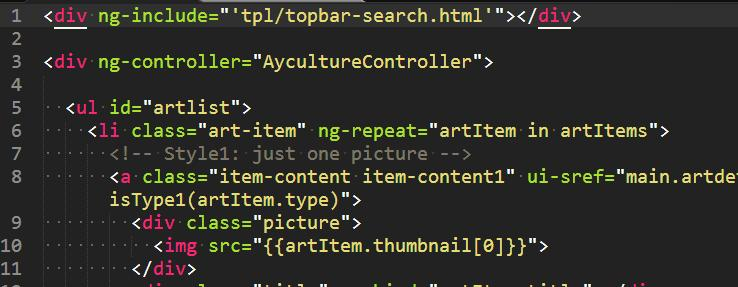
\includegraphics[width=10cm]{./img/tpl.jpg}
              \caption{模板页示例}
              \label{fig:tpl}
            \end{figure}

            路由的作用是:根据 url 控制加载相应的模板,通过 Angular 的 ui-router 模块实现,后面会具体讲解。如图 \ref{fig:router}

            \begin{figure}[H]
              \centering
              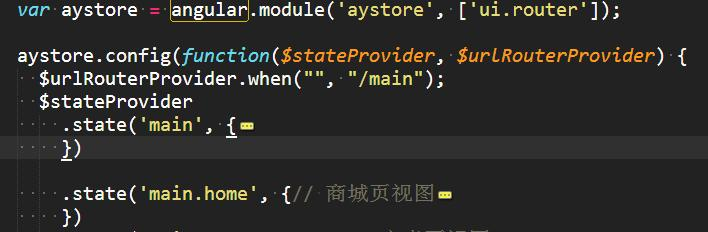
\includegraphics[width=10cm]{./img/router.jpg}
              \caption{路由示例}
              \label{fig:router}
            \end{figure}

    \section{工具}
      \label{sec:工具}
        \subsection{Sublime Text 3}
          \label{subsec:sublime_text_3}
            Sublime Text 3 是一款非常强大的编辑器,如图 \ref{fig:sublime}, 目前是我最喜欢的编辑器,有诸多的优点:
            \paragraph{漂亮} Sublime 本身的字体就很美观,目前我换成了 Source Code Pro 字体,这是目前我认为最漂亮的字体。
            \begin{figure}[H]
              \centering
              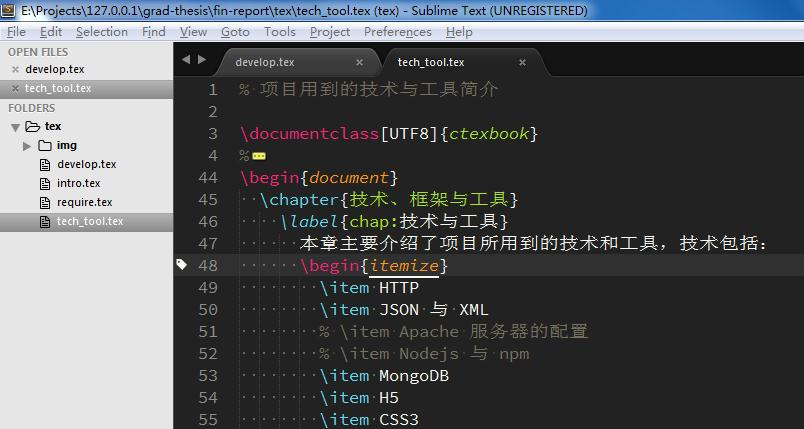
\includegraphics[width=8cm]{./img/sublime.jpg}
              \caption{Caption here}
              \label{fig:sublime}
            \end{figure}

            \paragraph{轻量} Sublime Text 3 的安装包只有 8 MB,即使在我安装了大量的插件(40 多个)后也不到 150MB,相比于 IDE 更加轻量,因此速度也是飞快。一个 IDE 至少几百兆甚至一两G, 大量的功能用不上,Sublime 的功能是根据需要来安装相应的插件,因此是按需索取,有更强的定制性。

            \paragraph{高效的操作} Sublime Text 官网中间就贴了一张动图,展示了 Sublime 的高效操作,如快速定位(文件、函数、某一行)、多光标编辑、快速选中单词和移动行等。

            \paragraph{插件系统、代码片段} Sublime 有着众多的插件,基本上可以打造任何编程语言的环境,语法高亮、实时纠错、代码片段等,让写代码快得飞起。

        \subsection{Chrome}
          \label{subsec:chrome}
            Chrome 是 Google 公司出品的浏览器,如图,
            \begin{figure}[H]
              \centering
              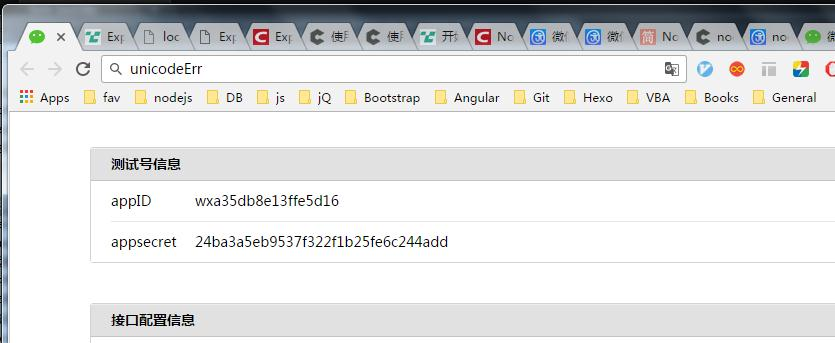
\includegraphics[width=8cm]{./img/chrome.jpg}
              \caption{Chrome 浏览器}
              \label{fig:chrome}
            \end{figure}
            功能强大,界面美观,兼容性好,有着强大的调试工具。Chrome 是前端开发必备的神器。浏览器的作用是渲染 HTML 和编译 JavaScript, HTML 在不断发展,不断增加新特性,这就要求浏览器的兼容性要好,同时 JavaScript 也在快速发展,浏览器此时作为编译引擎,性能要足够出色,Chrome 采用了 V8 引擎来编译 JavaScript ,是目前最快的编译引擎。同时,除了编译还要能够调试,Chrome 的调试功能也非常强大,如图 \ref{fig:chrome_debug}, 下面,我们就来详细谈谈 Chrome 的调试功能。
            \begin{figure}[H]
              \centering
              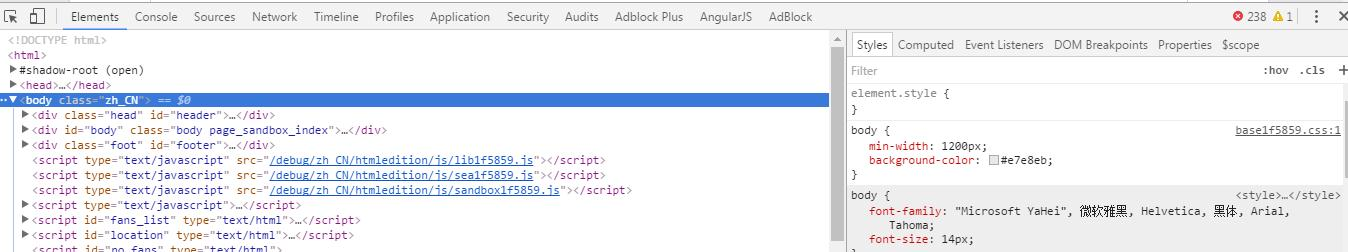
\includegraphics[width=10cm]{./img/chrome_debug.jpg}
              \caption{Chrome 的调试工具}
              \label{fig:chrome_debug}
            \end{figure}

            \subsubsection{Elements}
              \label{subsubsec:elements}
                我们看图 \ref{fig:chrome_debug} 中的几项菜单,第一个 Elements 是页面代码,可以方便的折叠和展开,坐上角的箭头一样的图标是用来审查(inspect)元素,如图 \ref{fig:cr_inspect},
                \begin{figure}[H]
                  \centering

                  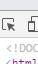
\includegraphics[width=3cm]{./img/cr_inspect.jpg}
                  \caption{Chrome 审查元素功能}
                  \label{fig:cr_inspect}
                \end{figure}
                翻译成捕捉更合适一点,因为它的功能是迅速定位元素在代码的位置,特别强大,如图 \ref{fig:cr_inspect1},
                \begin{figure}[H]
                  \centering
                  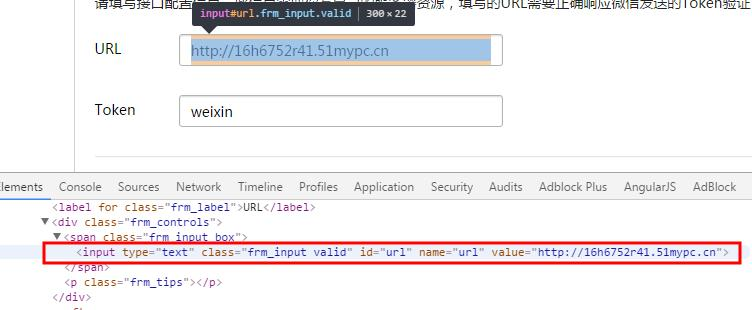
\includegraphics[width=8cm]{./img/cr_inspect1.jpg}
                  \caption{Chrome 定位元素的代码}
                  \label{fig:cr_inspect1}
                \end{figure}
                当点击审查元素的菜单后,我把鼠标移动到某个输入框上,Chrome 迅速为我定位到了其所在HTML代码处,同时右边还显示了对应的 CSS 样式,很强。
                \paragraph{title}
                \begin{figure}[H]
                  \centering
                  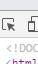
\includegraphics[width=8cm]{./img/cr_inspect.jpg}
                  \caption{Caption here}
                  \label{fig:figure1}
                \end{figure}

            \subsubsection{Console}
              \label{subsubsec:console}
                Console 即控制台,用于执行 javascript 语句和打印结果,如图 \ref{fig:cr_console},
                \begin{figure}[htbp]
                  \centering
                  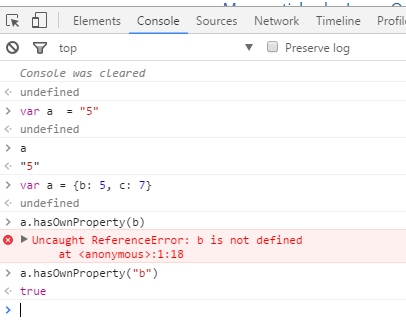
\includegraphics[width=8cm]{./img/cr_console.png}
                  \caption{控制台窗口}
                  \label{fig:cr_console}
                \end{figure}
                我一般用 Consolo 去测试一些 JavaScript 的方法、函数, dom 对象的一些方法以及测试 ajax 方法获取的数据是否正确。

            \subsubsection{Sources}
              \label{subsubsec:sources}
                Sources 是指加载的一些静态文件,如 html 文件,css 样式文件,图片,视频文件等,而加载的 js 文件可以进行断点调试,如图 \ref{fig:cr_sources}
                \begin{figure}[htbp]
                  \centering
                  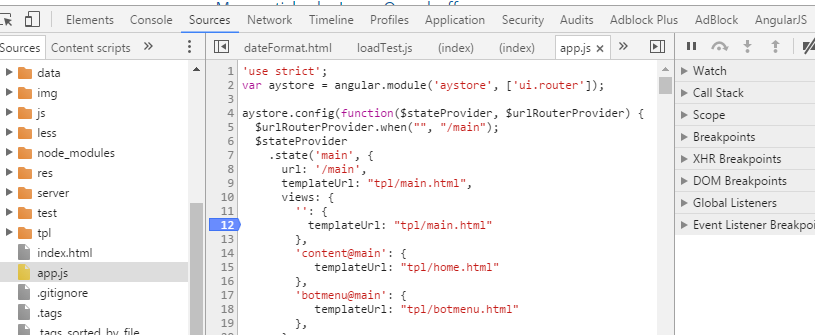
\includegraphics[width=8cm]{./img/cr_sources.png}
                  \caption{Sources}
                  \label{fig:cr_sources}
                \end{figure}
                变量的值还可以在当前执行的语句后显示出来。

            \subsubsection{Network}
              \label{subsubsec:network}



            \subsubsection{Application}
              \label{subsubsec:application}
                Application 一栏主要与缓存有关,如图 \ref{fig:cr_application}
                \begin{figure}[H]
                  \centering
                  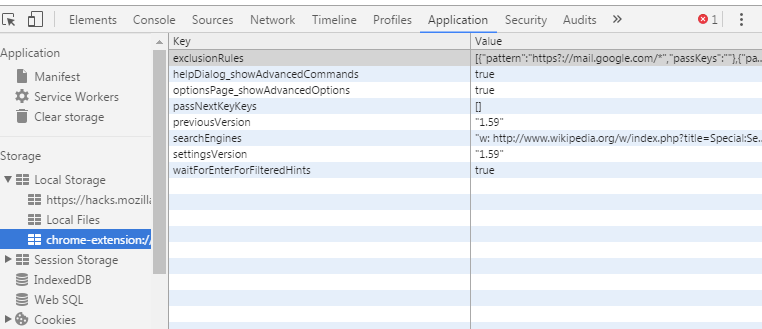
\includegraphics[width=8cm]{./img/cr_application.png}
                  \caption{application}
                  \label{fig:cr_application}
                \end{figure}
                左边 Application 目录下的 Manifest 保存了缓存文件的列表,Storage 目录下主要是本地存储技术,例如:
                \begin{itemize}
                  \item Local Storage
                  \item Session Storage
                  \item IndexedDB
                  \item WebSQL
                  \item Cookies
                \end{itemize}
                除了 Cookies,其他的存储方式都是 H5 新增的存储标准,容量一般都很大,例如 Local Storage 的容量可以达到 5MB, 而 Cookies 只有 4K,很多的网站开始尝试用 Local Storage 作为本地存储,而 IndexedDB 和 WebSQL 技术属于比较新的技术,还没有大面积使用。
                \par
                大量使用本地存储,对于服务器来说可以减轻负担,而对于客户端来说,减少了流量使用,提高了响应速度,Local Storage 我用来进行跨页数据传输问题,这只是方案之一,local Storage 的使用很方便,主要是 localStorage 对象,设置值用 localStorege.set('key', 'value') 或者 localStorege.key = value, 获取值用 localStorege.get('key') 或者 localStorege.key,因为 localStorage 也是一个对象,因此可以通过点或者中括号的方法获取或设置相应的值。
                \par
                以上介绍的功能是我在项目开发时常用的,调试非常方便,特别是在样式调试时的定位元素、实时修改属性值的时候,非常方便,而 JS 调试功能,如果是自己写的底层代码,即不用框架的话,调试起来是很方便的,会定位到相应的行,但是如果使用框架,问题就出来了,经常定位不到自己的代码中,而是定位到框架的代码中,如 angularjs 第 10500 行,此时就很头痛,只能把错误信息拿到网页去查询,这样的调试耗去了我大部分时间,针对框架调试的问题,我还没有找到好的方法。
                \par
                总之,Chrome 的调试工具无比强大,用好它可以大大缩短开发进度。

        \subsection{微信 Web 开发者工具}
          \label{subsec:微信_web_开发者工具}
            微信 Web 开发者工具是用来做微信开发的,实际上移动端的开发也可以用,如图 \ref{fig:wxweb}
            \begin{figure}[H]
              \centering
              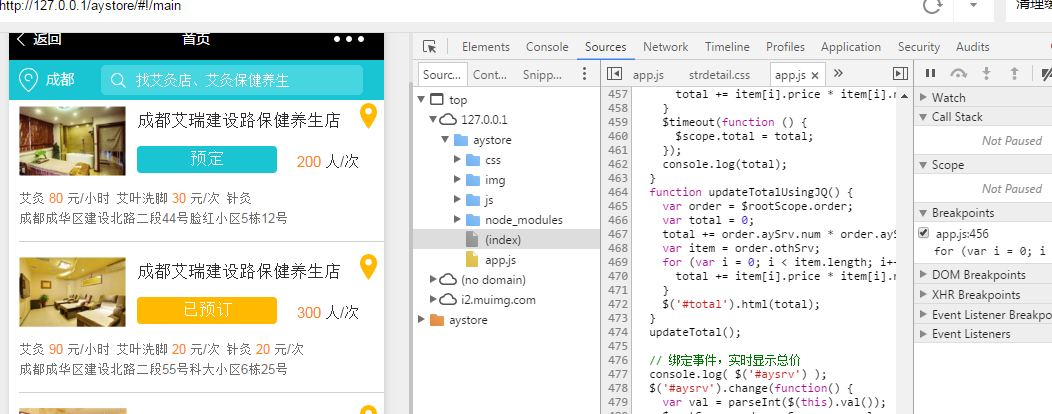
\includegraphics[width=8cm]{./img/wxweb.png}
              \caption{Caption here}
              \label{fig:wxweb}
            \end{figure}
            微信 Web 开发者工具采用的就是 Chrome 的调试工具,只不过只针对移动页面而已,不过也有其他的扩展,如 JSSDK 功能等。

        \subsection{Git}
          \label{subsec:git}
            Git 一款强大的版本控制工具,最早是用于 Linux 开发,由 Linux 系统的开发者 linus Trovals 研发。版本控制系统的目标是控制项目的版本,它可以记录你的每一次提交,因此你可以很方便的回到历史的版本,而不用去创建大量的备份,可以创建分支,团队协作开发等。Git 相对于其他的版本控制系统,更强大的地方在于本地仓库,每台设备都有一模一样的本地版本,不用担心中央服务器突然崩溃的问题。我个人用 Git 主要是用于版本同步,我有时在公司实习写的代码要和寝室的代码同步,简单的几行命令就可实现。













    \section{小结}
      \label{sec:小结}

\end{document}

